\vspace{-0.4em}
\section{MATERIALS AND METHODS}\label{sec:matmet}
\subsection{Macrophages embryos}\label{sec:macrophages}
Five hundred and forty one time frames with dimensions
$(n_h, n_w, n_d) = (512, 672, 3)$ and two  fluorescent channels
(red = GFP-Moesin, green = Clip-GFP) were
acquired as described in \cite{Stramer2010}.
%The green channel illustrates the variations of shape in the cells.
Figure \ref{fig:mat-evol} shows the temporal variation of one cell.
Four basic shapes, Fig. \ref{fig:mat-cellframe}, can be recognised in the data:
\textbf{circles or ellipses, drops} (one pointy edge like a water drop),
\textbf{bi-drops} and \textbf{tri-drops} (similar to a drop but with more than one pointy edge).
%For the analysis of the shape, a large collection of synthetic images that model cell shapes was created. This dataset is described next.
\begin{figure}[hbpt]
\vspace{-0.1cm}
    \centering
    \subfigure[Full frame.]{
        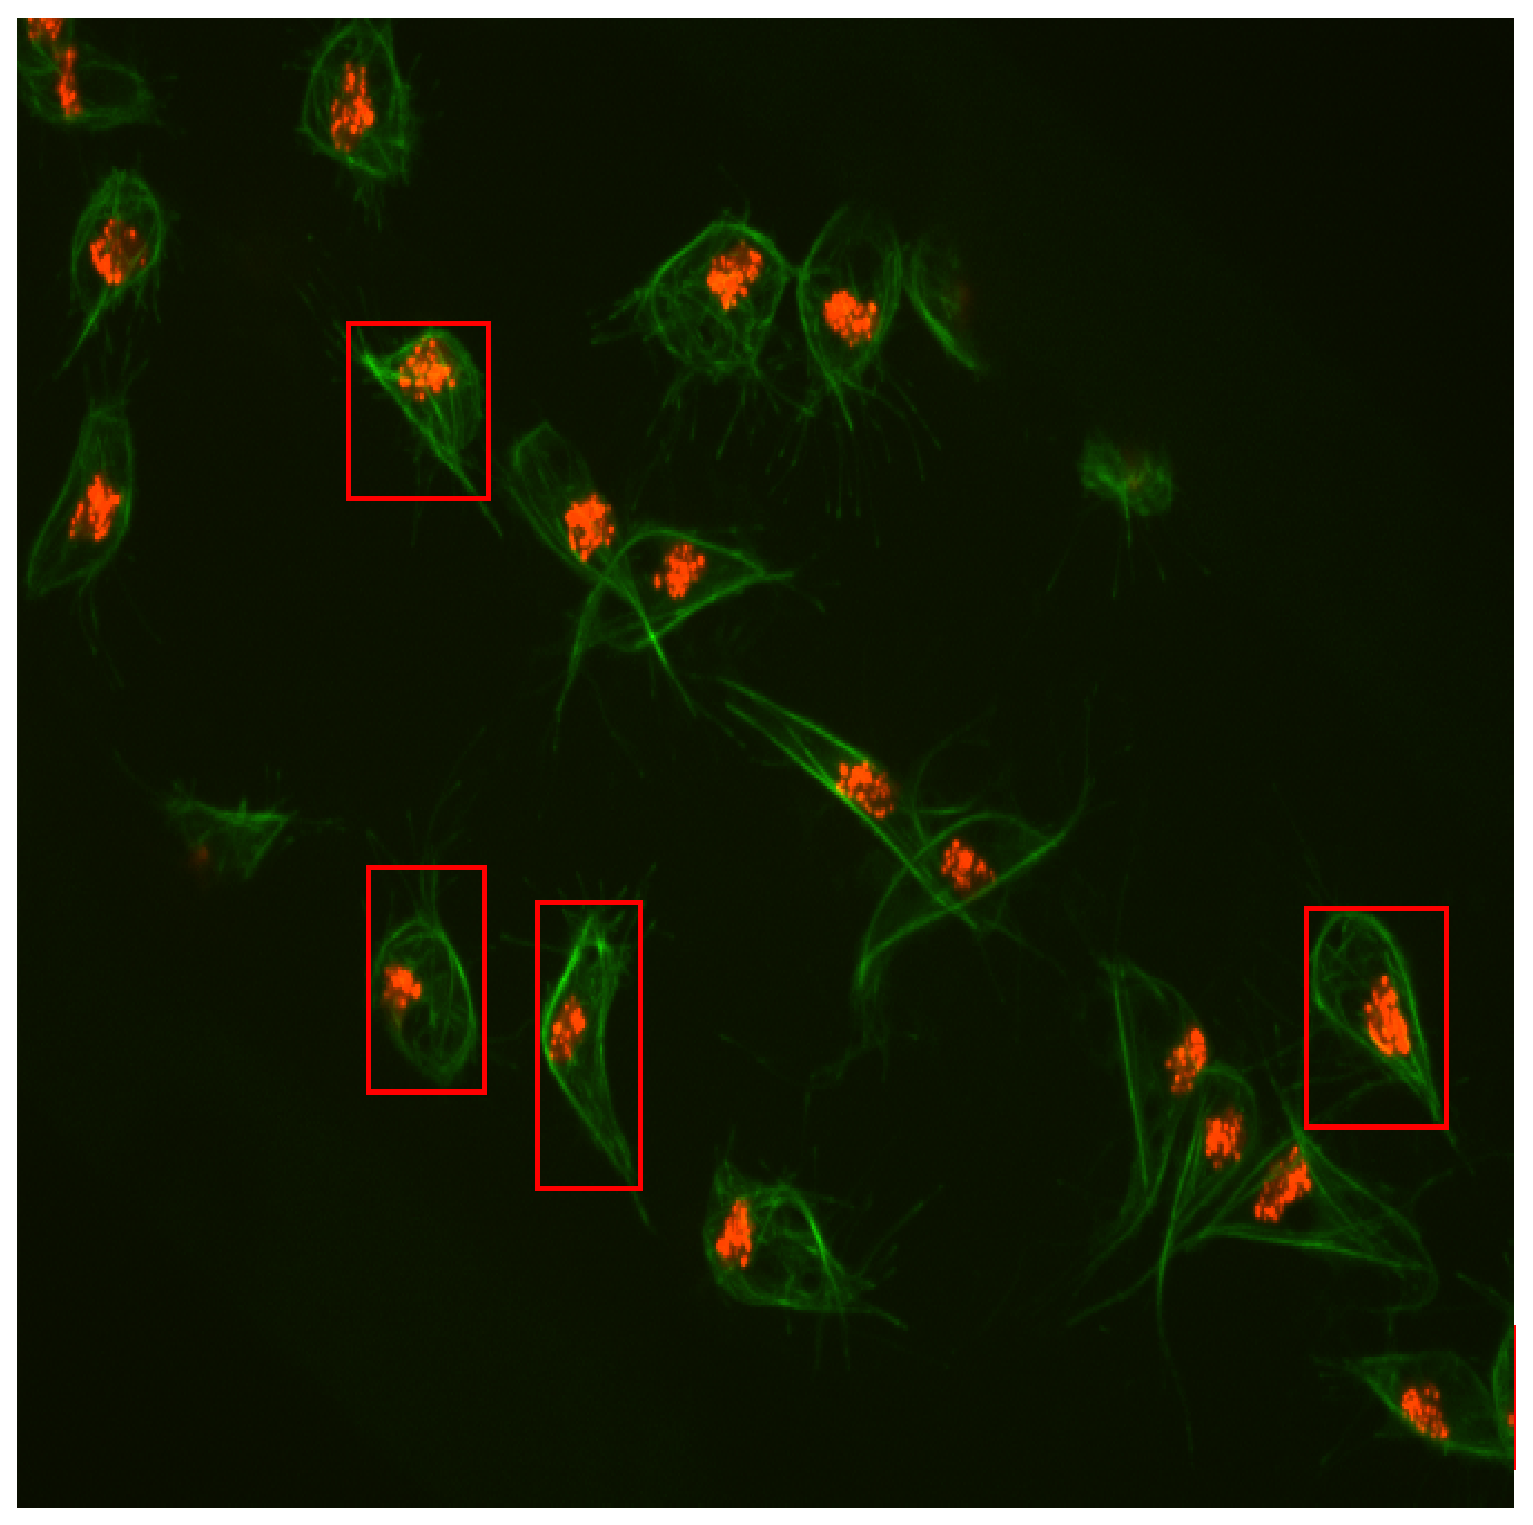
\includegraphics[width=0.2\textwidth]{mat-fig1-1}
    }
    \subfigure[ROIs with basic shapes
    ]{
        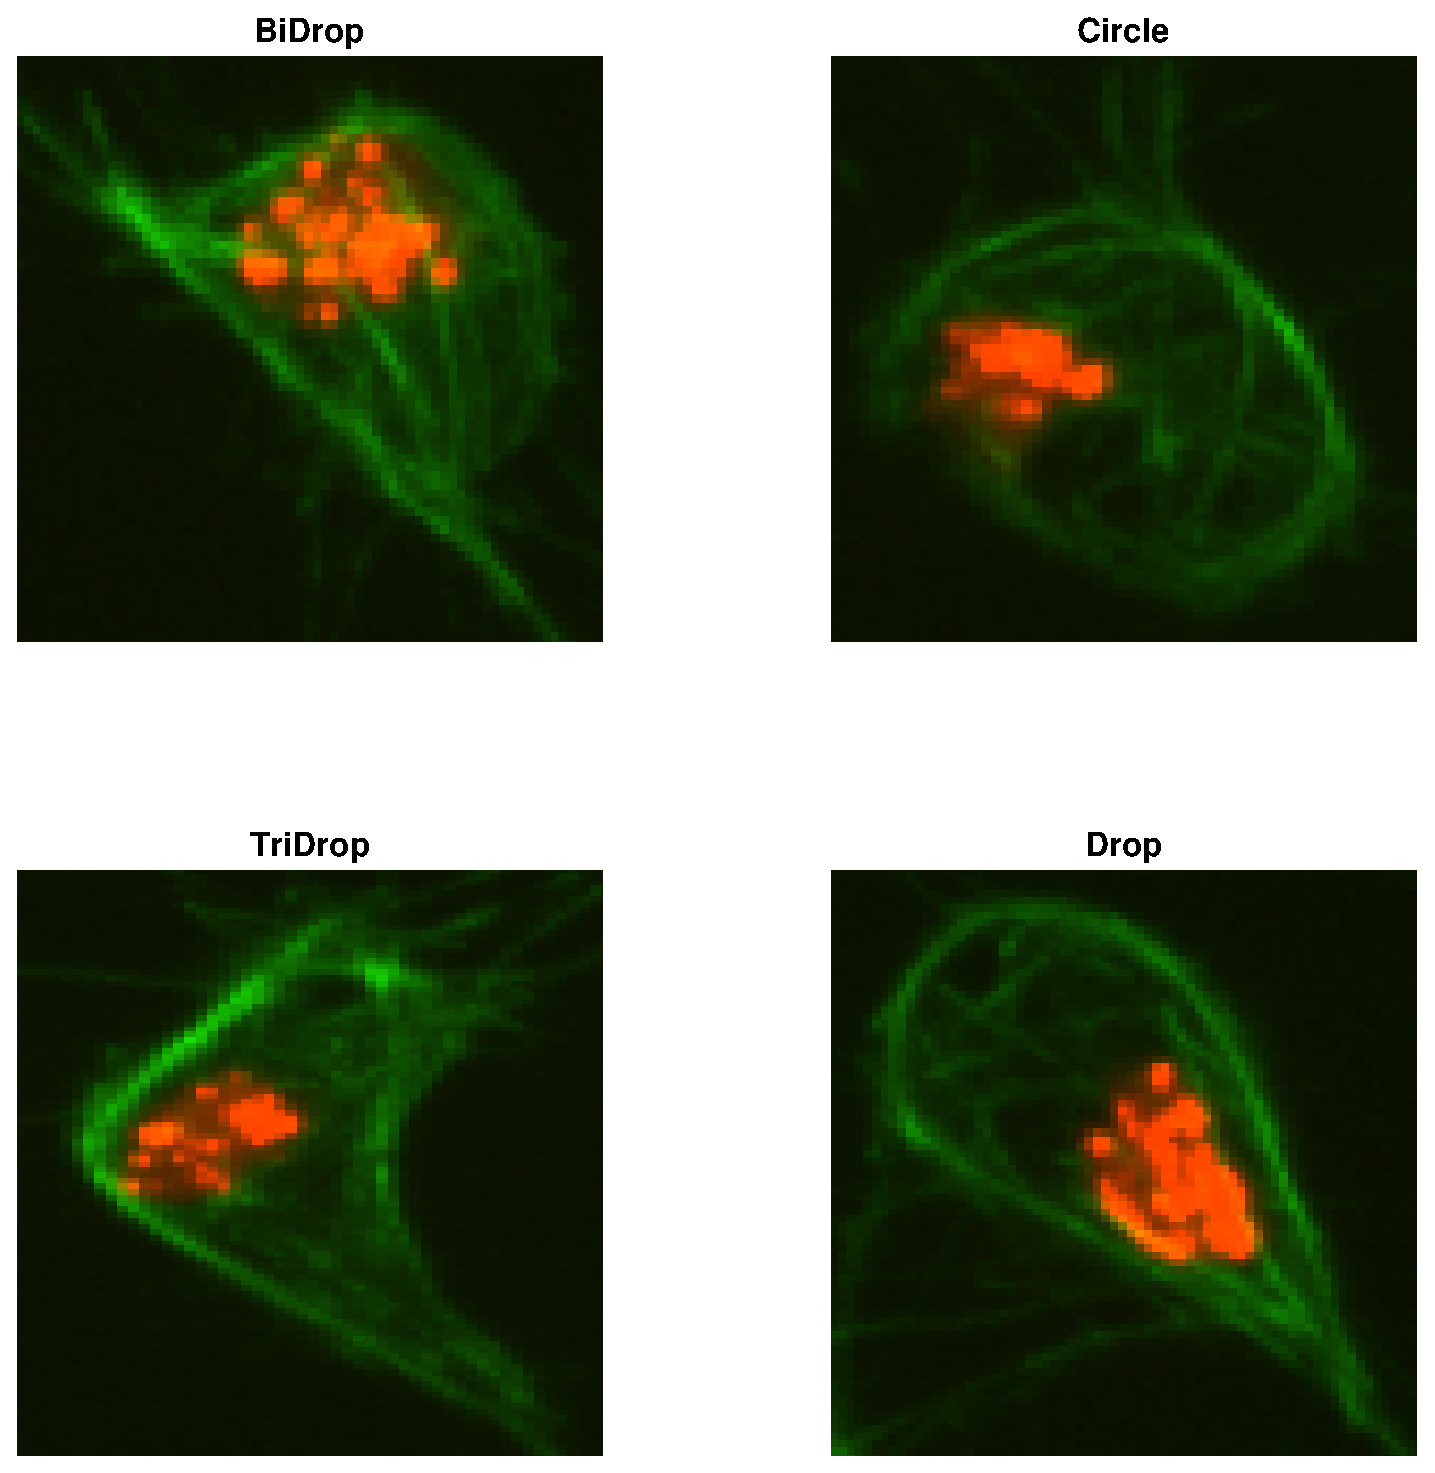
\includegraphics[width=0.2\textwidth]{mat-fig1-2}
    }
    \caption[One representative time frame %Example of cell shapes in the macrophages dataset.
    ]{
      \small
      One representative time frame where all basic shapes can be recognised.
      (a) Full frame  with (red) squares highlighting the cells
      of interest. (b) Detail of each cell.
      }
    \label{fig:mat-cellframe}
\end{figure}
\vspace{-1em}
\begin{figure*}[hbpt]
    \centering
    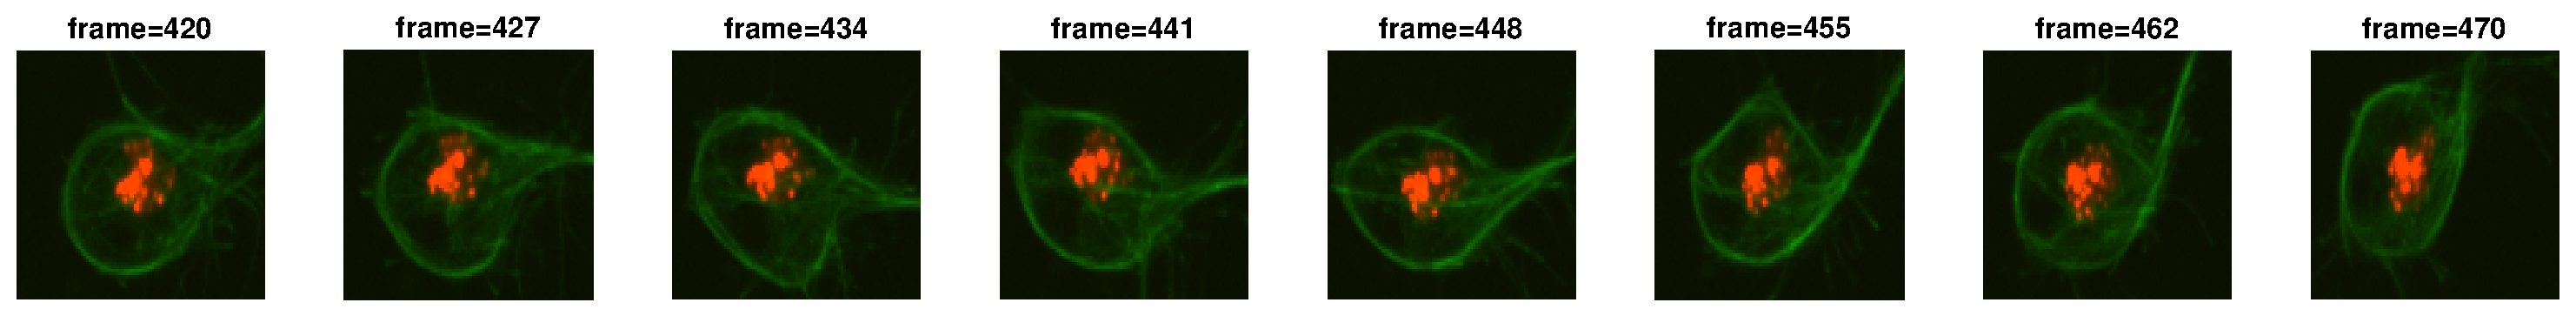
\includegraphics[width=0.9\textwidth]{mat-fig2}
    \caption[Evolution of a cell shape in time.]{
    \small
    Evolution of a cell shape in time. The cell is shown
    in 8 different instances from 50 consecutive time frames.
    }
    \label{fig:mat-evol}
\end{figure*}
\vspace{-1em}
\subsection{Synthetic data}
A collection of 1000 images of basic shapes was generated with control
points joined by cubic splines whose independent variable ranged in
$\tau\in[0,2\pi]$
. %to make the curve revolve around itself.
Let $\left\{Y^{\star}_i\right\}_{1}^{N} = \{(x_{1,i}, y_{2,i})\}_{1}^{N}$,
be a collection of $N$ control points of a basic shape such that
$Y^{\star}_i \sim \mathcal{N}\left( \mu^{\star}_i, \sigma^{\star}_i \right) $.
The value of $N$ depends on the type of basic shape: \textbf{circle} has 4,
\textbf{drop} has 7, \textbf{bi-drop} has 8 and \textbf{tridrop} has 10.
To model the variations in the cells' shapes, within their basic categories,
the control points are distributed Normal. The control points are joined with a
spline that then produces the \textbf{boundary} of the shape, $\boundy$, which then
models that of a segmented cell (Fig. \ref{fig:mat-synth}).
% illustrates the basic mean shapes that were generated from 200 different examples.
\begin{figure}[hbpt]
    \centering
    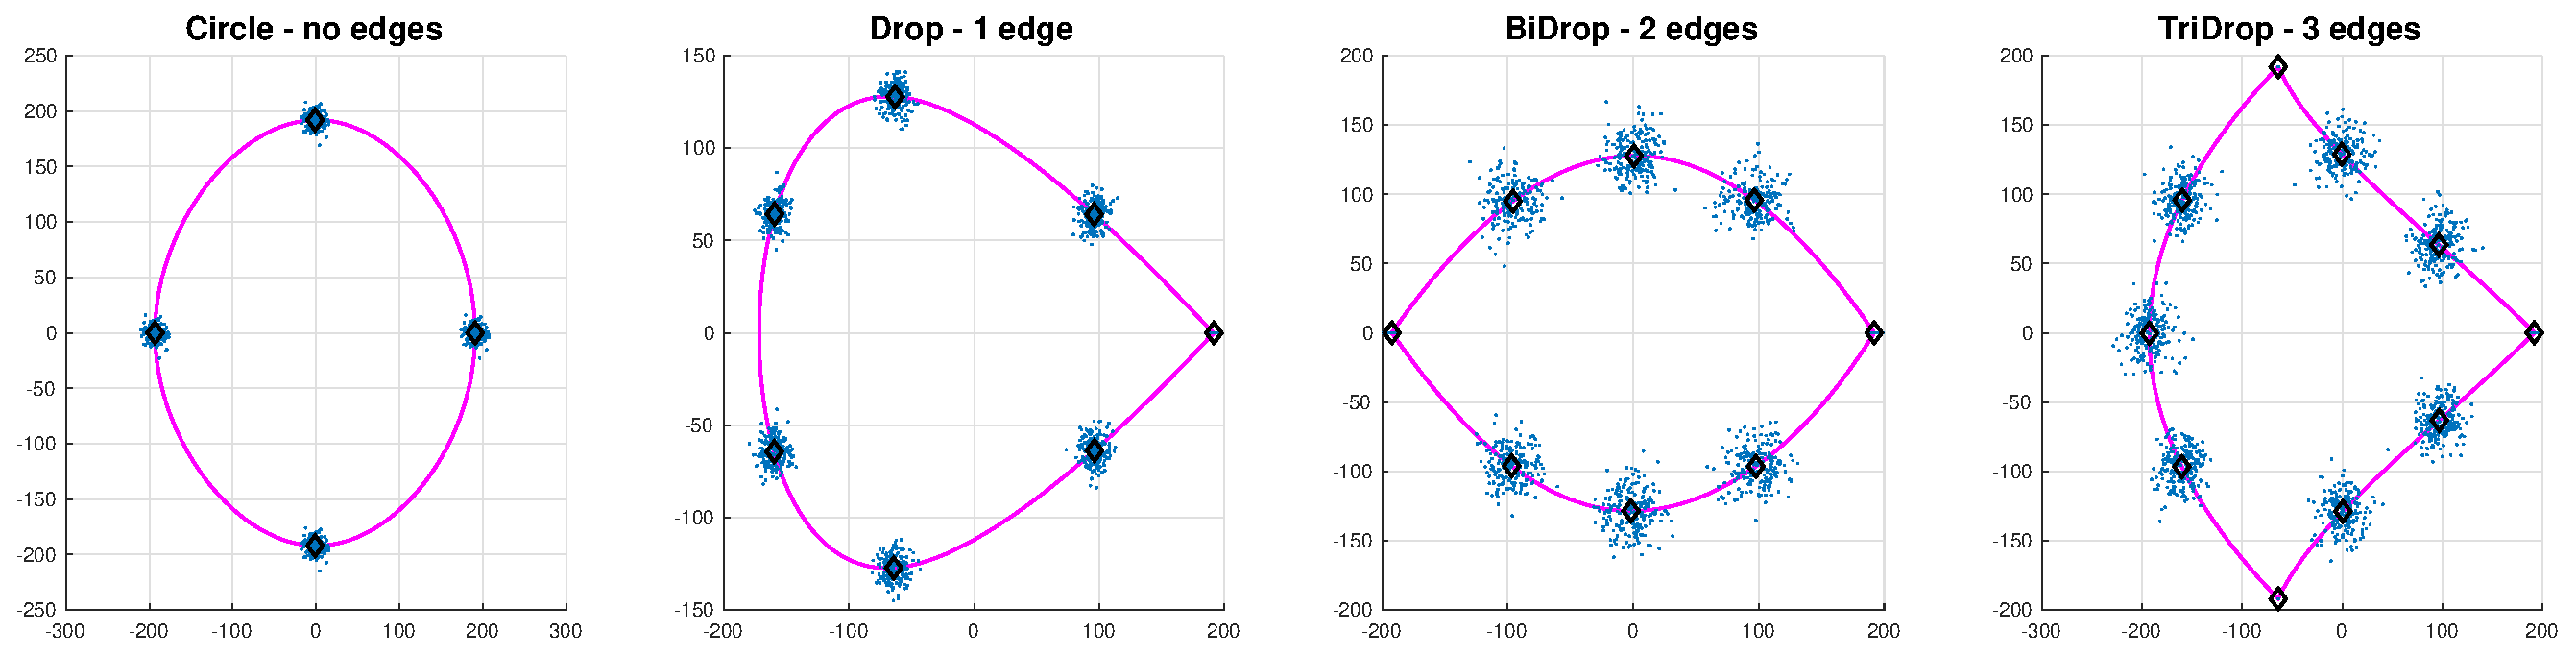
\includegraphics[width=0.5\textwidth]{mat-fig3}
    \caption[Synthetic generation of random basic shapes.]{\small
    Synthetic generation of random basic shapes.
    Per shape, 200 cases were generated.
    The control points are shown in blue($\cdot$).
    The mean shapes are presented in magenta($-$); and the
    mean control points are represented in black($\diamond$).
    }
    \label{fig:mat-synth}
\end{figure}
\vspace{-1.5em}
\subsection{Shape tracking methodology}
The shape of the cells was extracted from the green channel whilst the red
channel was used to distinguish between individual and overlapping cells.
%which were not analysed in this work.
Both channels were low pass filtered
with a 5$\times$5 Gaussian kernel and then segmented by Otsu
thresholding \cite{Otsu1979}.
Finally, a morphological opening with a disk structural element
($r=3$) was performed
to smooth the edges and remove noise. As reported in \cite{solislemus2017},
this segmentation can be used to distinguish between overlapping groups of
cells called \emph{clumps}.
%This work is focused in tracking the non overlapping cells.
This work focuses in tracking the non overlapping cells.
The main functionality presented is a framework in which a cell
shape can be tracked
through a curve evolution algorithm.
The PhagoSight package  \cite{Henry2013} was used to track the movement
of the nuclei through time using the keyhole algorithm, and the segmentation of
the green channel was used to determine which nuclei were involved in a clump.
Clumps were removed from the analysis.
The tracking produced unique
labels for each of the tracks detected, as well as the
position of each nuclei at each point in time. Each track is represented by
$\track_{j}$, with $j=1,2,\cdots,M$ being the number of tracks.
Each $\track_{j}$ contained the information regarding the
positions of the centroid of the nuclei $\{\mathbf{x}_{j,k}\}_{k=1}^T$ as well as
the time frames where the track was present $t_{j,0}, \cdots, t_{j,k}, \cdots,
t_{j_{0, T-1}}$ for the $T$ consecutive time frames.
%It is clear that $1\leq t_{j,0} < \cdots < t_{j_{0, T-1}} \leq T_0 = 541$.
For simplicity, a time frame of an arbitrary track $\track$ is shown as $t_k$.

Given a track $\track$, the shape of a cell $\boundy_{k+1}$
at any time $t_{k+1}$ can be determined by the shape
of the previous frame $\boundy_{k}$, and the position change
%$\mathbf{x}_{k+1} - \mathbf{x}_{k}$
from $t_k$ into $t_{k+1}$ of the red nuclei. Let $\bar{\boundy_{k}}$ be the
shape $\boundy_{k}$ when moved onto the position $\mathbf{x}_{k+1}$.
The shape $\boundy_{k+1}$ will be determined by \textbf{evolving}
$\bar{\boundy_{k}}$ the shape from the previous time frame,
where $\image_k$ corresponds to the image of the $k_{th}$ time frame
(Algorithm \ref{tab:shapeevo}). Every iteration of the
algorithm involves loading the known frame $t_k$, the position information
from the unknown frame $t_{k+1}$, performing the evolution from
$\bar{\boundy}_{k+1}$ to $\boundy_{k+1}$ and obtaining the region properties
of the new cell shape, these include
(i) the \emph{orientation},
%defined as the angle from the x-axis to major axis;
(ii) the ratio of the minor and major axes (\emph{aspect ratio}),
(iii) the \emph{solidity}, and
%the ratio of the area of $\boundy$ and the area of the convex hull that covers it;
(iv) the \emph{equivalent diameter}.
%of the circle with the same area as the region.
%\vspace{-0.5em}
\begin{algorithm}
\KwIn{Track: $\track$, time frames: $(t_0:t_{T-1})$}
$t_k \gets t_0$;\\
$(\image_k, \vecx_k) \text{load frame information at } t_k$;\\
$\boundy_k \gets \text{get boundary}(\image_k)$;\\
\For{$t_{k+1}$ in time frames} {
    $t_{k+1} \gets t_k+1$;
    $(\image_{k+1},\vecx_{k+1}) \gets \text{load frame at } t_{k+1}$;
    $d_k \gets \vecx_{k+1}-\vecx_k$;\\
    $\bar{\boundy}_{k+1} \gets \text{move boundary}
    (\boundy_k, d_K)$;\\
    $\boundy_{k+1} \gets \text{evolve}(\image_{k+1}, \bar{\boundy}_{k+1})$;\\
    save$(\boundy_{k+1}, \text{regionprops}(\boundy_{k+1}))$;\\
    $t_k \gets t_{k+1}$;\\
    $\boundy_k \gets \boundy_{k+1}$;\\
}
\caption{\small {\sc shape evolution} Tracks shape of cells in a single track.}
\label{tab:shapeevo}
\end{algorithm}
%\vspace{-1em}
The \textbf{evolve} function in Algorithm \ref{tab:shapeevo} implements
the Chan-Vese active contour \cite{chanvese,whitaker1998} method in \matlab.
The function uses
%the moved boundary
$\bar{\boundy}$ as initialisation
and is able to change its parameters based on one of three
states: Shrink, Grow, or Normal (Table \ref{tab:acparams}).
The active contour runs once, with a set of parameters,
then the area of the output is compared to the area of the input.
The parameters would be adjusted to contract or expand the shape
and the active contour is re-run.
To avoid an excessive segmentation leaking/contraction,
the area of the output was kept within $\pm5$\% of the previous
frame's area.
\vspace{-0.5em}
\begin{table}[hbpt]
    \centering
    \caption{\small
    Parameters used of the active contour function based on the desired
    state required. The parameters were chosen empirically through numerous
    tests.
    }
    \begin{tabular}{c|ccc}
    \hline
    State	& Iterations &	Smooth factor &	Contraction bias\\
    \hline
    \textbf{Normal} & 50 & 1.5 & -0.1 \\
    \textbf{Shrink} & 100 & 1.25 & 0.10 \\
    \textbf{Grow} & 200 & 1.00 & -0.25 \\
    \hline
    \end{tabular}
    \label{tab:acparams}
\end{table}
\vspace{-2em}
\begin{figure}[hbpt]
    \centering
    \subfigure[Junctions.]{
    \includegraphics[width=0.12\textwidth]{meth-fig4-1}
    \label{fig:meth-anglegram-1}
    }
    \subfigure[Anglegram and max intensity projection.]{
    \includegraphics[width=0.28\textwidth]{meth-fig4-2.pdf}
    \label{fig:meth-anglegram-2}
    }
    \caption{
    \small
    Description of the original junction detection by \emph{anglegram}.
    The junctions detected on a pair or ellipses is shown in (a),
    where the boundary of the overlap is blue(- -) and the
    junctions in magenta ($\diamond$). In (b), the \emph{anglegram} is
    displayed in a plane and the \emph{MIP} is represented
    along the boundary points. Detection of junctions are shown in magenta
    ($\diamond$).}
    \label{fig:meth-anglegram}
\end{figure}
\vspace{-1em}
\subsection{Shape analysis through \emph{Anglegram}}
The \emph{anglegram} \cite{solislemus2017} is a matrix, which describes multiscale
angle variation of a shape.
For each one of the ordered points $\mathbf{p}_i\in\boundy$,
the inner angles of every point are computed for every separation and the maximum
intensity projection (\emph{MIP}) per columns is calculated.
To detect clumps, the angles of interest were those larger than %$180^{\circ}$.
one standard deviation (\emph{std}) above the mean of the MIP.
In this work, a similar idea is explored, but for \emph{acute} angles,
using the minimum intensity projection (\emph{mIP}) and the threshold is
one \emph{std} below the mean.
Implementing the anglegram matrix involves the detection
of junctions that correspond to the corners of the analysed boundary.
Figure \ref{fig:meth-anglegram} illustrates the junction detection functionality
of the anglegram. The method works as reported in \cite{solislemus2017}, with
two alterations: (i) resizing the anglegram to have 64 rows to reduce noise,
and (ii) taking the \emph{mIP} of the first half
columns, as the final columns are lower by the definition of the inner point
angle measurements. The corner detection method was tested on 70,000 randomly
generated boundaries of the different types of shapes. Then, the corners were
detected on the shapes of the cells being tracked for a qualitative assessment.
\begin{figure}[hbpt]
    \centering
    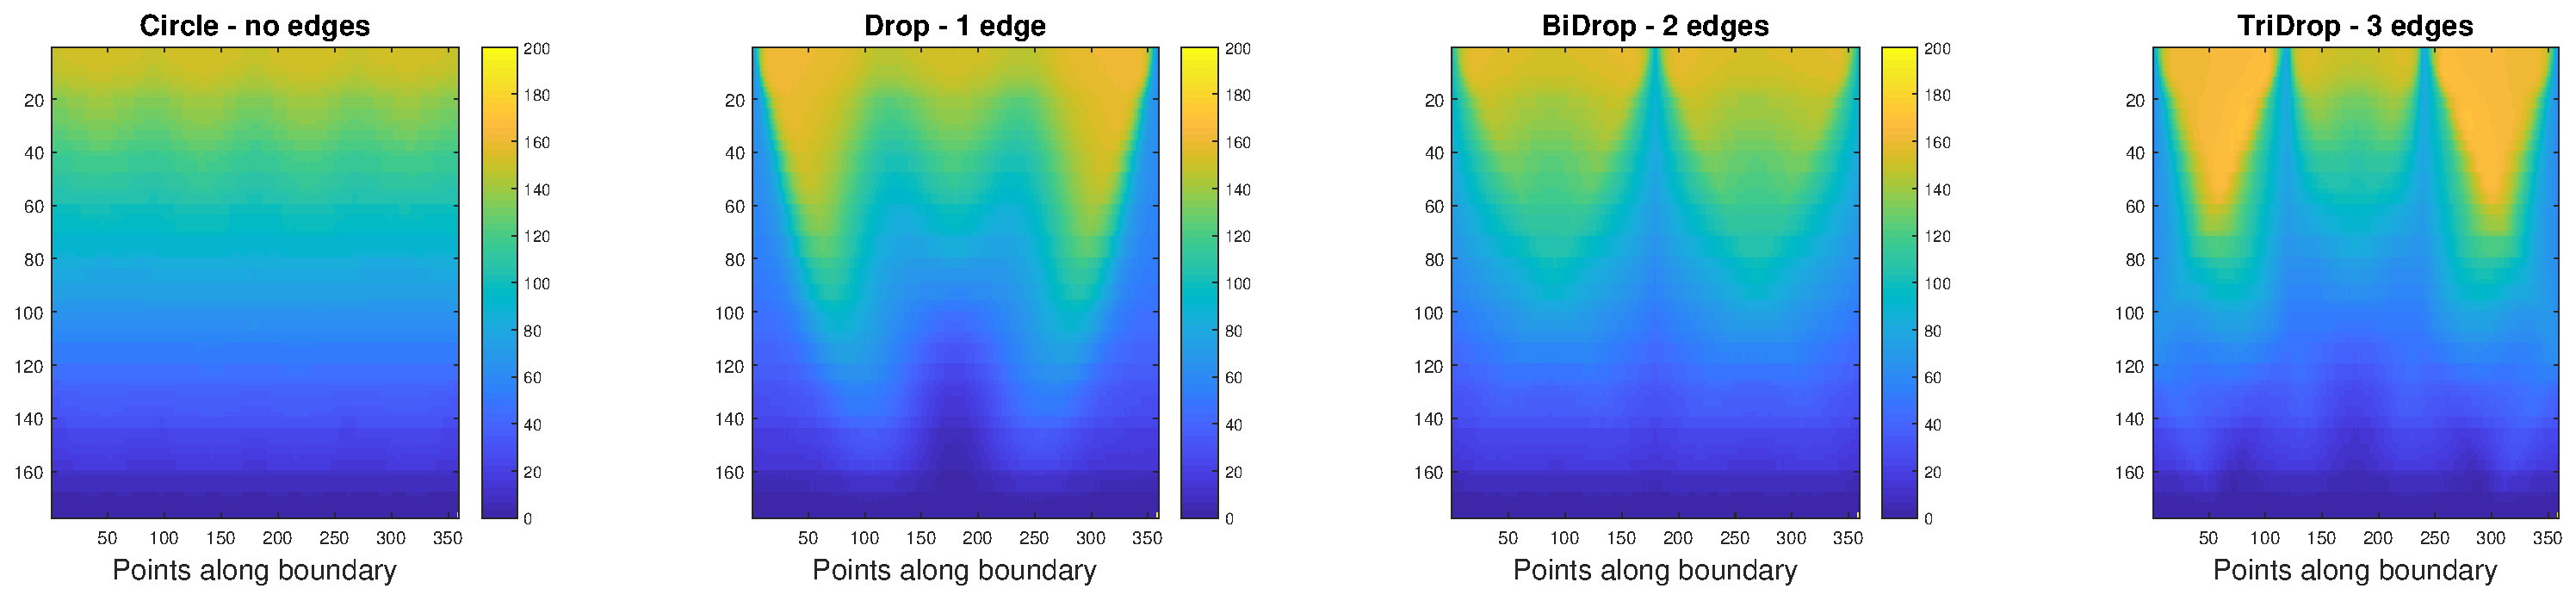
\includegraphics[width=0.45\textwidth]{mat-fig2-2}
    \caption[Anglegram on mean basic shapes from Figure \ref{fig:mat-synth}.]
    {\small
    Anglegram on mean basic shapes from Figure \ref{fig:mat-synth}.
    The anglegram matrix was calculated and transposed for visualisation
    purposes. %Each of the basic mean shapes is represented.
    Left to right: \textbf{circle, drop, bidrop} and
    \textbf{tridrop}.
    }
    \label{fig:agshapes}
\end{figure}
\vspace{-0.5em}
